% \def\course{Math 228}
%
%
%
%
% \title{Discrete Mathematics: An Open Introduction}
% %{\large Course Notes for Math 228 at the University of Northern Colorado}
%
%
%
%
% \author{Oscar Levin}
%
% \date{Fall 2015}
%
% \begin{titlingpage*}



\documentclass[10pt]{article}

\usepackage{amsmath, amssymb}
\usepackage{url}
\usepackage{xcolor}
\usepackage{tikz}
\usepackage{mdframed}
\usepackage[papersize={8.5in,11in}, hmargin={1.5in, .5in}, textheight=10.5in]{geometry}

\definecolor{bg}{HTML}{DBA639}
\definecolor{txt}{HTML}{252D49}
\definecolor{ltxt}{HTML}{B4B07C}
\definecolor{boxbg}{HTML}{38544C}
\pagecolor{bg}

\usepackage[T1]{fontenc}
\usepackage{newpxtext}
\usepackage[vvarbb,cmintegrals,cmbraces,bigdelims]{newpxmath}
\usepackage[scr=rsfso]{mathalfa}% \mathscr is fancier than \mathcal
\linespread{1.04}         % adds more leading (space between lines)
% quantifiers look strange, so change those back to normal:
	\DeclareSymbolFont{mysymbols}{OMS}{cmsy}{b}{n} %note we make the figures bold to better match newpx.  Replace the ``b'' with an ``m'' to undo this.
	%\SetSymbolFont{mysymbols}  {bold}{OMS}{cmsy}{b}{n}
	%\DeclareSymbolFont{myoperators}   {OT1}{cmr} {m}{n}
	%\SetSymbolFont{myoperators}{bold}{OT1}{cmr} {bx}{n}
	\DeclareMathSymbol{\forall}{\mathord}{mysymbols}{"38}
	\DeclareMathSymbol{\exists}{\mathord}{mysymbols}{"39}
	%\DeclareMathSymbol{\pm}{\mathbin}{mysymbols}{"06}
	%\DeclareMathSymbol{+}{\mathbin}{myoperators}{"2B}
	%\DeclareMathSymbol{-}{\mathbin}{mysymbols}{"00}
	%\DeclareMathSymbol{=}{\mathrel}{myoperators}{"3D}


\begin{document}

\pagestyle{empty}

\color{txt}


% ~
\tikz[remember picture, overlay]{
\draw[fill, boxbg, thick] (current page.south east) rectangle +(-8.5in, 3in);
% \draw[fill, boxbg, thick] (current page.north west) rectangle +(8.5in, -.75in);
\draw[fill, txt, thick] (current page.north west) rectangle +(1in, -11in);
}

~
\vskip 1.5in

\begin{center}

\resizebox{.8\linewidth}{!}{\textbf{\scshape Some Abstract Algebra}}

\vskip 1in


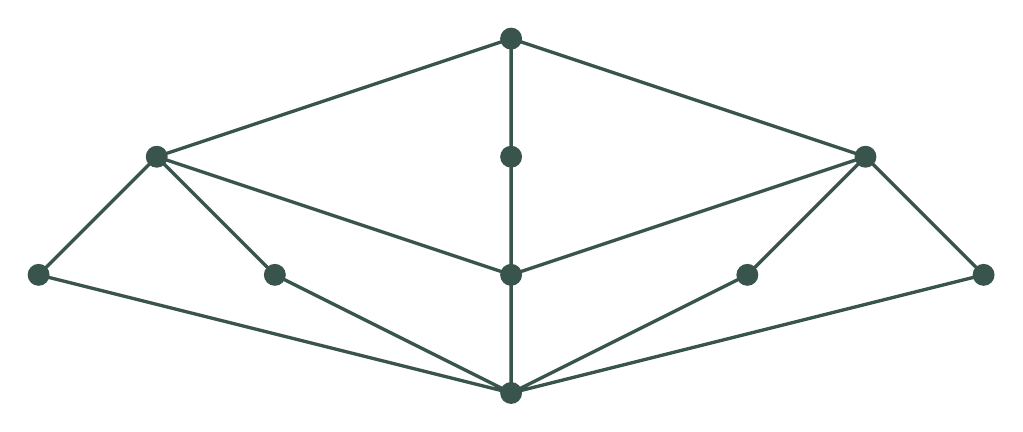
\begin{tikzpicture}[scale=1.5]
	\coordinate (h9) at (0,0);
	\coordinate (h8) at (4,1);
	\coordinate (h7) at (2,1);
	\coordinate (h6) at (0,1);
	\coordinate (h5) at (-2,1);
	\coordinate (h4) at (-4,1);
	\coordinate (h3) at (3,2);
	\coordinate (h2) at (0,2);
	\coordinate (h1) at (-3,2);
	\coordinate (h0) at (0,3);

	\draw[color=boxbg, very thick] (h0) -- (h1) -- (h4) -- (h9) -- (h8) -- (h3) -- (h0) -- (h2) -- (h6) -- (h9) -- (h5) -- (h1) -- (h6) -- (h3) -- (h7) -- (h9);
	\foreach \i in {0,...,9}{
	\draw[fill=boxbg, color=boxbg] (h\i) circle (2.5pt);
	}
\end{tikzpicture}

\vskip .75in

\resizebox{.65\linewidth}{!}{\scshape A Primer and Interactive Workbook}

\vskip 2in
\vskip 1in
\end{center}


\begin{center}
\color{ltxt}
\resizebox{.8\linewidth}{!}{\scshape Richard Grassl \quad - \quad Tabitha Mingus}
\end{center}
% \vskip 1.1in
%
% \resizebox{.25\linewidth}{!}{\scshape 2nd Edition}
\vfill
% \begin{flushright}
% 	\color{ltxt}
% 	% \resizebox{.25\linewidth}{!}{\textit{Open Math Books}}
% 	% \resizebox{.25\linewidth}{!}{$\mathbb{O}\mathrm{p}\mathrm{e}\mathrm{n}$ $\mathbb{M}\mathrm{a}\mathrm{t}\mathrm{h}$ $\mathbb{B}\infty\mathrm{k}\mathrm{s}$}
% 	\resizebox{.25\linewidth}{!}{$\mathbb{O}\mathrm{p}\mathrm{e}\mathrm{n}$ $\mathbb{M}\mathrm{a}\mathrm{t}\mathrm{h}$ $\mathbb{B}\mathrm{oo}\mathrm{k}\mathrm{s}$}
% 	% \resizebox{.25\linewidth}{!}{$\mathbb{O}{p}{e}{n}$ $\mathbb{M}{a}{t}{h}$ $\mathbb{B}\infty{k}{s}$}
% \end{flushright}

\clearpage

%\includepdf[pages=-,pagecommand={\thispagestyle{empty}}]{frontmatter/cover2}
%
%

\end{document}






%\addtocontents{toc}{\protect\thispagestyle{plain}}
